% Please use the skeleton file you have received in the
% invitation-to-submit email, where your data are already
% filled in. Otherwise please make sure you insert your
% data according to the instructions in PoSauthmanual.pdf
\documentclass{PoS}

\newcommand{\khzcm}{\mathrm{kHz/cm^2}}
\newcommand{\hzcm}{\mathrm{Hz/cm^2}}
\newcommand{\ohmcm}{\mathrm{\Omega\,cm}}
\newcommand{\DT}{\mathrm{\Delta T}}


\title{Fast timing measurement for the CMS RPC Phase II upgrade}

\ShortTitle{CMS RPC Phase II upgrade}

\author{\speaker{Maxime Gouzevitch} on behalf of the CMS collaboration\\
        Univ Lyon, Universit\'e Lyon 1, CNRS/IN2P3, IPN-Lyon F-69622, Villeurbanne, France\\
        E-mail: \email{mgouzevi@ipnl.in2p3.fr}}

%\author{Another Author\\
%        Affiliation\\
%        E-mail: \email{...}}

\abstract{With the increase of the LHC luminosity foreseen in the coming years many detectors currently used in the different LHC experiments will be dramatically impacted and some need to be replaced. The new ones should be capable not only to support the high particle rate but also to provide time information to reduce the data ambiguity due to the expected high pileup.

The Resistive Plate Chambers (RPC) using low-resistivity Bakelite are proposed to equip the very forward region of the CMS detector. In their single-gap version they can stand rates of few $\khzcm$. New electronics equipped with excellent timing precision measurement ($< 150$\,ps) are being developed to read out the RPC detectors from both side of the strips to allow good spatial resolution along them. The absolute time measurement, determined by RPC signal (around 0.8 ns) will also reduce the data ambiguity due to the highly expected pileup at the Level 1 trigger and help to identify Heavy Scalar Charged Particles.

The principle of the measurement, and the implementation of innovative front-end electronic boards (PETIROC front-end ASIC, wave-union TDC and PCB design) will be discussed. First results from test beams at the Gamma Irradiation Facility and the SPS at CERN would also are presented.
}

\FullConference{The 39th International Conference on High Energy Physics (ICHEP2018)\\
		4-11 July, 2018\\
		Seoul, Korea}

\begin{document}

\section*{Introduction}

In the present CMS detector, all the muon stations are equipped with three kinds of muon detectors. Drift Tubes (DT) and RPC detectors are used in the barrel region.  The endcap region up to pseudorapidity $|\eta| = 2.5$ is instrumented by the Cathode Strip Chambers (CSC), while RPC chambers stop at $|\eta| = 1.8$.
To guarantee a redundancy in this region and improve the muon trigger efficiency it is planned to add new chambers during long shut-downs LS2 (2019-2020) and LS3 (2024-2026) of the LHC. The projected increase of the LHC luminosity  up to $5-7 \cdot 10^{34}$\,cm$^{-2}$s$^{-1}$ during the High Luminosity phase of LHC (HL-LHC) suggests that new detectors with high rate capability are needed~\cite{upgrade}.

Figure \ref{fig.upgrade} summarizes the project of the upgrade of the muon spectrometer. 
Gaseous electron multiplier (GEM) detectors are proposed to equip the first of these four high $\eta$ muon stations and improved RPC chambers (iRPC) the last two stations (RE3/1 and RE4/1). In this region, the expected rate during the HL-LHC program shall not exceed 2\,$\khzcm$ including a safety factor of 3 \cite{upgrade}. The new stations are required to detect muons with an efficiency above 95\% and to sustain a total integration charge of 1\,C/cm$^2$ corresponding to the full period of operations during the HL-LHC program. A good intrinsic time resolution would improve the rejection of background hits and low transverse momentum tracks. It would also help to resolve ambiguities in the endcap trigger
for identification of multiple tracks and allows reconstruction of slowly moving Heavy Stable Charged Particles.

\begin{figure}
  \begin{center}
    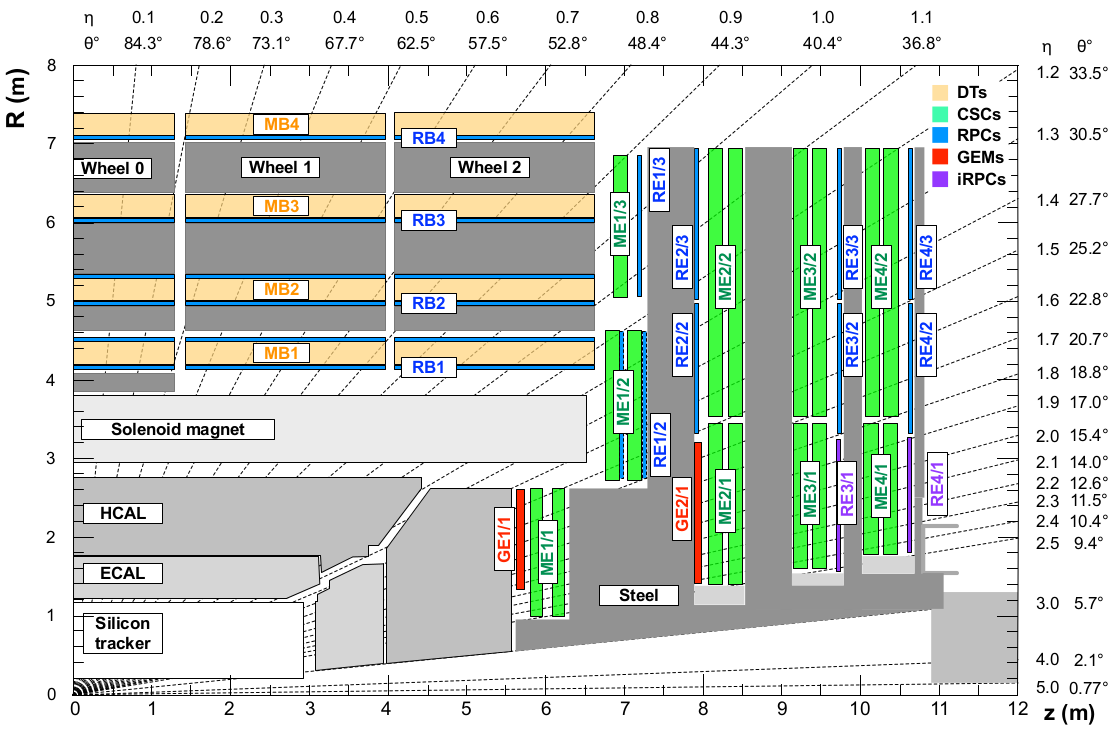
\includegraphics[width=0.50\textwidth]{figs/rpclayout.png}
  \end{center}
 \caption{Upgrade project of the CMS muon spectrometer.} \label{fig.upgrade}
\end{figure}

\section{Description of the iRPC project}

The classical RPC chambers of CMS are doublet RPC detectors each made of two $2.0$\,mm HPL electrodes, with a typical bulk resistivity of $1-6 \cdot 10^{10}\,\ohmcm$ and separated by a gas gap of the same thickness. The electronics reading those chambers is sensitive to a minimal charge left by a muon of $150$\,fC \cite{Chatrchyan:2008zzk}.
They were shown to be operational up to 600\,$\hzcm$, but above their efficiency was declining. To sustain a 3 times larger rate we have to modify some of the parameters.

A reduction of the electrodes resistivity to $1-3 \cdot 10^{10}\,\ohmcm$ and thickness to $1.4$\,mm would improve the total evacuation flow of the charge. The chamber could sustain a higher background. A thinner gas gap of $1.4$\,mm would reduce the produced charge per background hit and reduce the stress on the electrodes with effect due to aging. The drawback of this approach is a smaller charge left by a muon. Therefore a more sensitive electronics is required to keep the sensitivity as high as possible.

Two types of electrodes fulfilling the HL-LHC requirements were proposed: aluminum doped glass \cite{Gouzevitch:2016pcr} and modified HPL electrodes. The latter solution was privileged by the Collaboration as a more familiar one with respect to the present RPC system after a first set of tests \cite{upgrade}.

The baseline read out electronics foreseen for this project is based on a thin ($0.6$\,mm) Printed Circuit Board (PCB), 160 cm long, equipped with 48 pickup strips of the same length inserted between two HPL gaps. In order to maximize charge induction between the gaps and the strips, we must minimize the thickness of the Flame Resistant 4 (FR4) layers of the PCB. Considering the large size of the PCB, the thickness of FR4 of $300$\,$\mu$m on each side of the strips seems to be the lowest acceptable value in terms of mechanical rigidity and handling capabilities.
Two PCBs would read out a full chamber covering an azimuthal region of $20^{\circ}$. The strips of an average pitch of $0.75$\,cm are read out from both ends, the one that is located at the low radius of the iRPC ring (LR) and the other at the high radius (HR). Both signals are fed into the same Front-End Board (FEB) in such a way that the time difference between them $\DT = {\rm T}_{\rm HR} - {\rm T}_{\rm LR}$ largely cancels out jitter effects. Subsequently $\DT$ can be directly related to the along-strip space resolution. 

To maximize the signal collected on both ends of the strip, the FEB impedance is precisely matched to the one of the strips. It was observed that strip impedance is defined by the distance between the strips and the Faraday cage enclosing the chamber and is very dependent on the exact chamber design. In the configuration proposed for iRPC, an impedance of $44\,\Omega$ was determined.

The FEB is carrying a fast front-end ASIC, PETIROC2 \cite{PETIROC2}, a 32 channels version developed in SiGe technology. It hosts a preamplifier with a $1$\,GHz bandwidth and gain of 25 associated with a fast programmable comparator. The comparator output for each PETIROC channel is fed into an Altera cyclone II FPGA hosting the time-to-digital conversion module.

The electronics calibration procedure starts from the alignment of the pedestals of all the comparators inside a PETIROC chip, and more generally among all the PETIROCs. We define then a global threshold for all the comparators in such a way that the amount of noise does not exceed 5\,$\hzcm$ as requested by the CMS trigger constraints.

Full size prototypes of the iRPC detector were built in 2017 to test two different ways to connect the PCB to the FEB: using $50$\,$\Omega$ coaxial cables running outside of the Faraday cage (referred to as Coax-scheme) or return strips embedded into the PCB (Return-scheme). It was observed that the Return-scheme prototype is better protected from the grounding and pickup noise than the Coax-scheme one. During the test beams we had to use a threshold of 81 (108)\,fC for Return-scheme (Coax-scheme) prototypes. More details on the electronics can be found in Ref.~\cite{Combaret}.

\section{Chamber characterization}

The prototypes were extensively tested in cosmic rays and then in two sessions of test beams in the Gamma Irradiation Facility (GIF++) \cite{Jaekel:2014yya} during 6 weeks. A low intensity muon beam was hitting the chamber together with a uniformly distributed photon background generated by a $^{137}$Cs source.

A muon is considered as detected if it was seen by at least one strip from both sides within a time window around the expected arrival of the trigger that is delayed by $600$\,ns due to the length of the cables. The size of this time window is defined as $\pm3\sigma_{\rm T}$, with $\sigma_{\rm T} \approx 2$\,ns as shown in Fig. \ref{fig.T}. This value is defined by a convolution of the trigger jitter, scintillator size and the intrinsic jitter of the chamber. We have measured the latter to be $\sigma_{\rm HR} = 0.8$\,ns by comparing the difference of the time of arrival of the signal between the HR side of the two chambers. A similar one is observed between the two LR sides. The obtained resolution can be then be divide by $\sqrt{2}$ assuming the chambers electronics to be identical and uncorrelated (see Fig. \ref{fig.T}). If many strips are localized in space and time, they are gathered together in clusters. The typical cluster size is around $1.2-1.3$ strips, depending on the pitch and background rate, guaranteeing a transverse space resolution much better than $1$\,cm.

\begin{figure}
  \begin{center}
    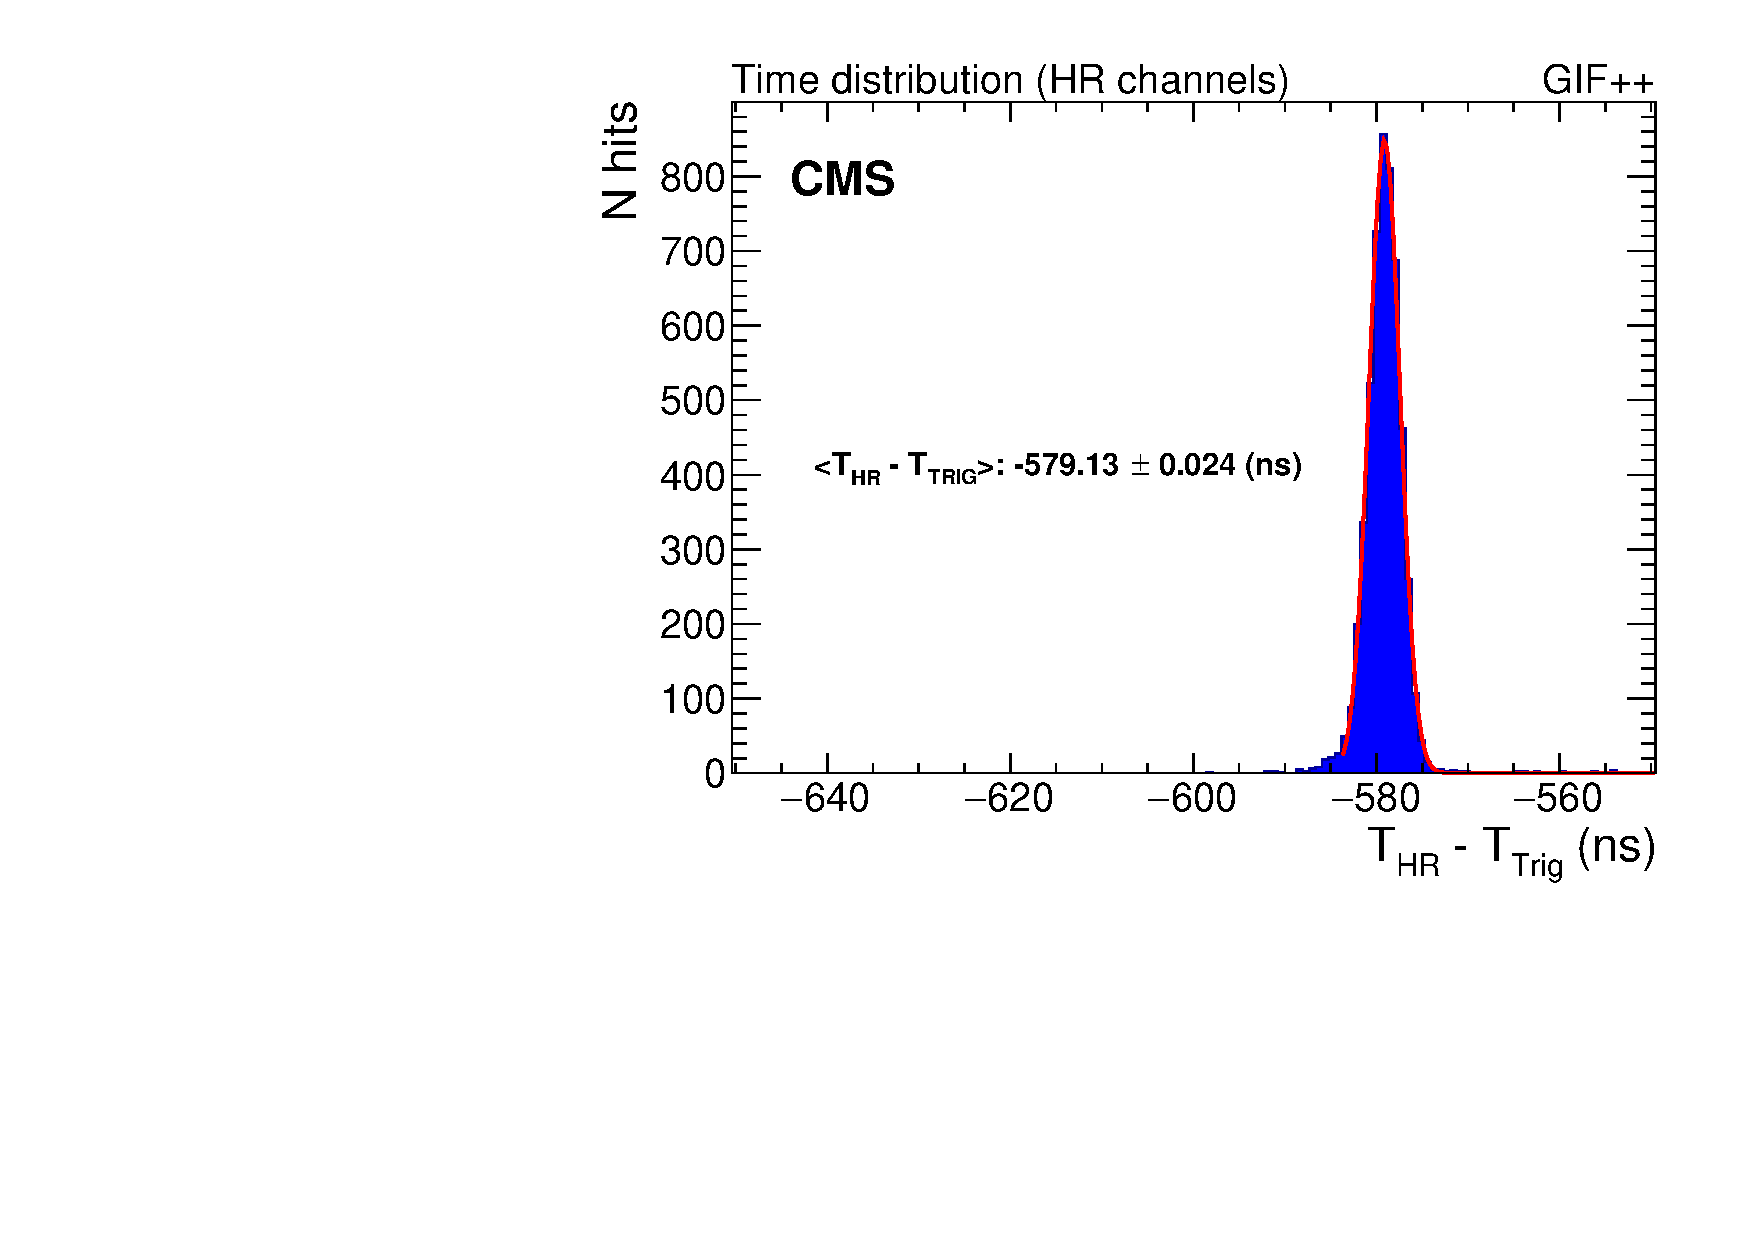
\includegraphics[width=0.40\textwidth]{figs/HR.pdf}
    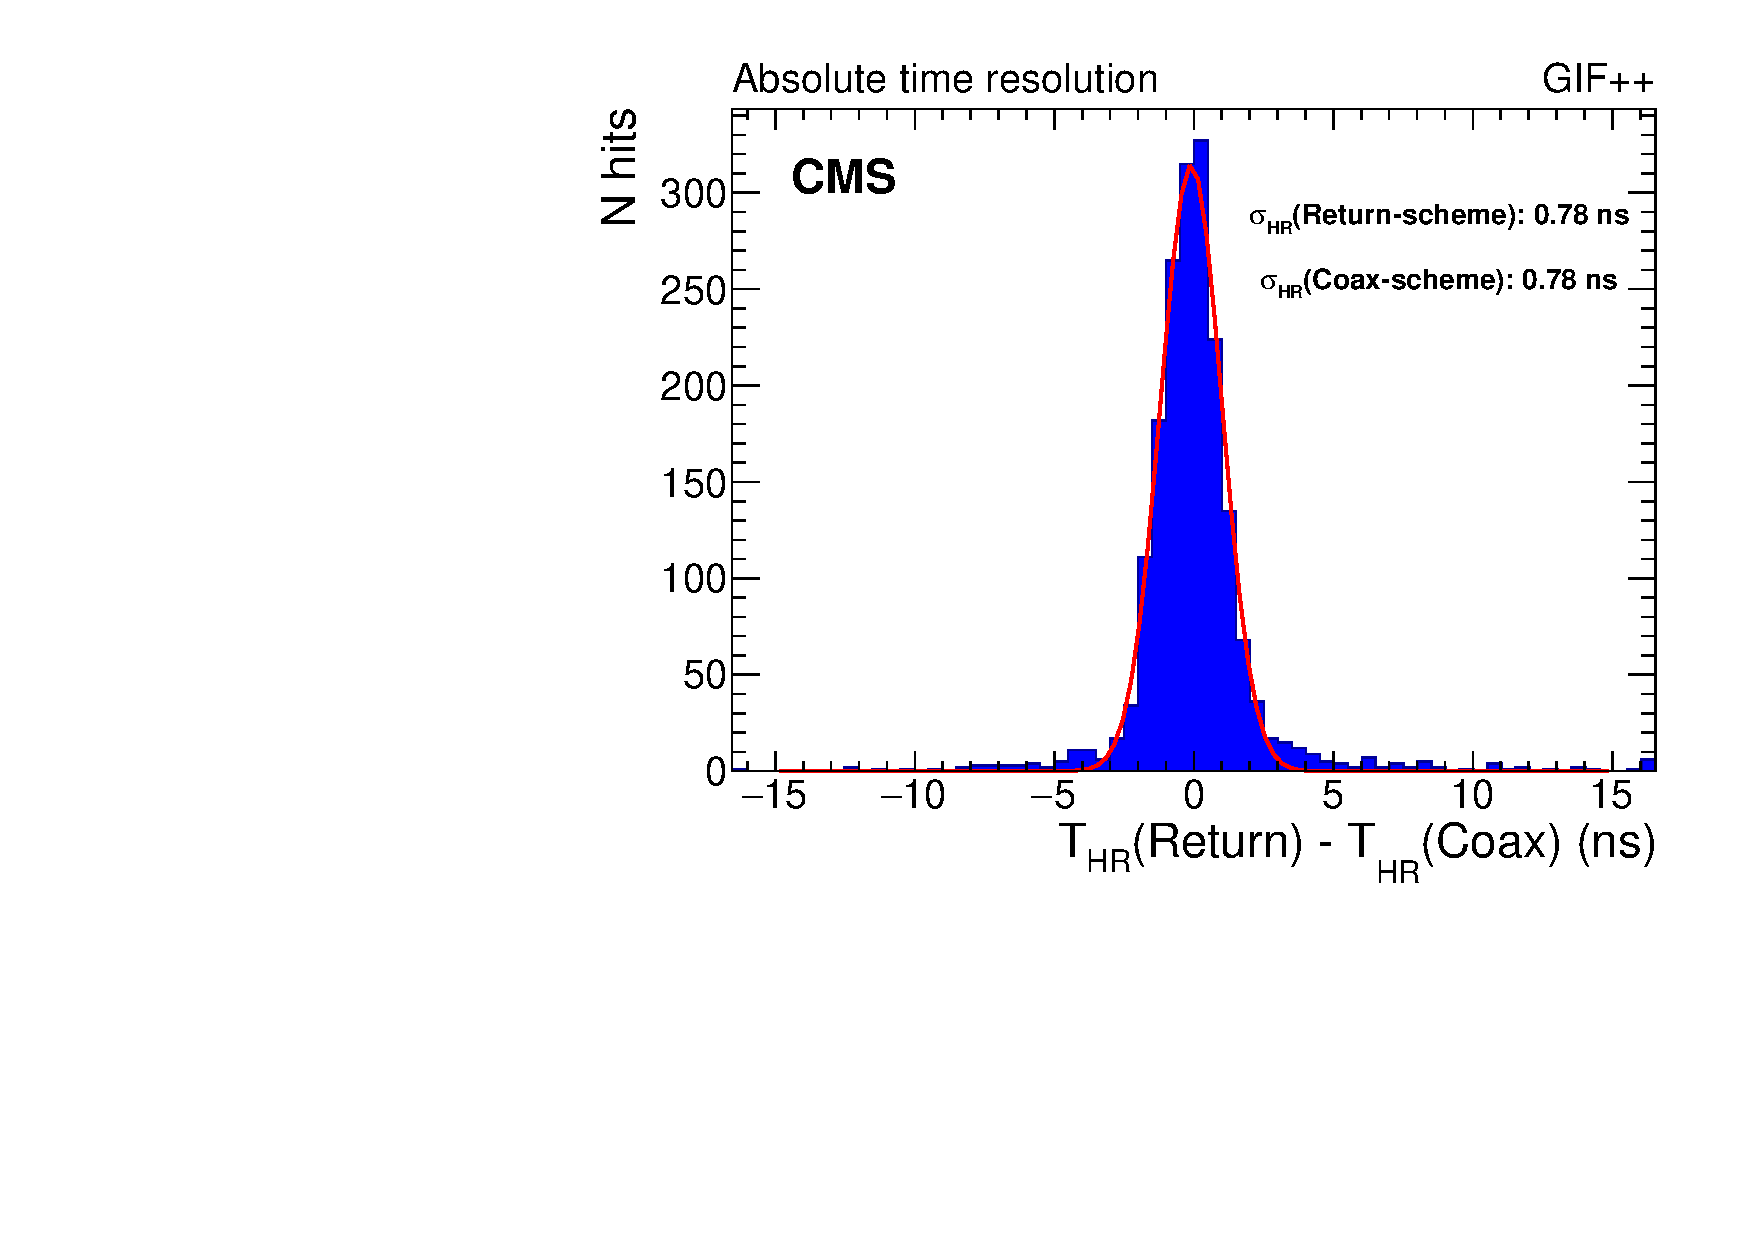
\includegraphics[width=0.40\textwidth]{figs/DELTA_T.pdf}
  \end{center}
 \caption{Time difference between the arrivals of the signal from HR side and from the trigger logic (left): the Gaussian fit defines the time jitter. Difference in time between the HR side of the Coax-scheme and Return-scheme prototypes used to measure the intrinsic time jitter of the chambers $\sigma_{\rm HR}$.} \label{fig.T}
\end{figure}

The presence of muons was also identified by an independent telescope made of 4 scintillators with an effective area well inside the detector acceptance. The efficiency of the chambers was then measured comparing the number of identified muons with those who left a signal in the chamber. Figure \ref{fig.eff} shows efficiencies for different rates that are defined as the number of clusters seen by the chamber. We observe that the efficiency of the chamber stays above 95\% up to $2\,\khzcm$ as required by the project specifications. Both prototypes show similar efficiencies. The chamber can be operated at a voltage as low as 7.3 kV for low background and 7.6 kV for maximum rate.


\begin{figure}
  \begin{center}
    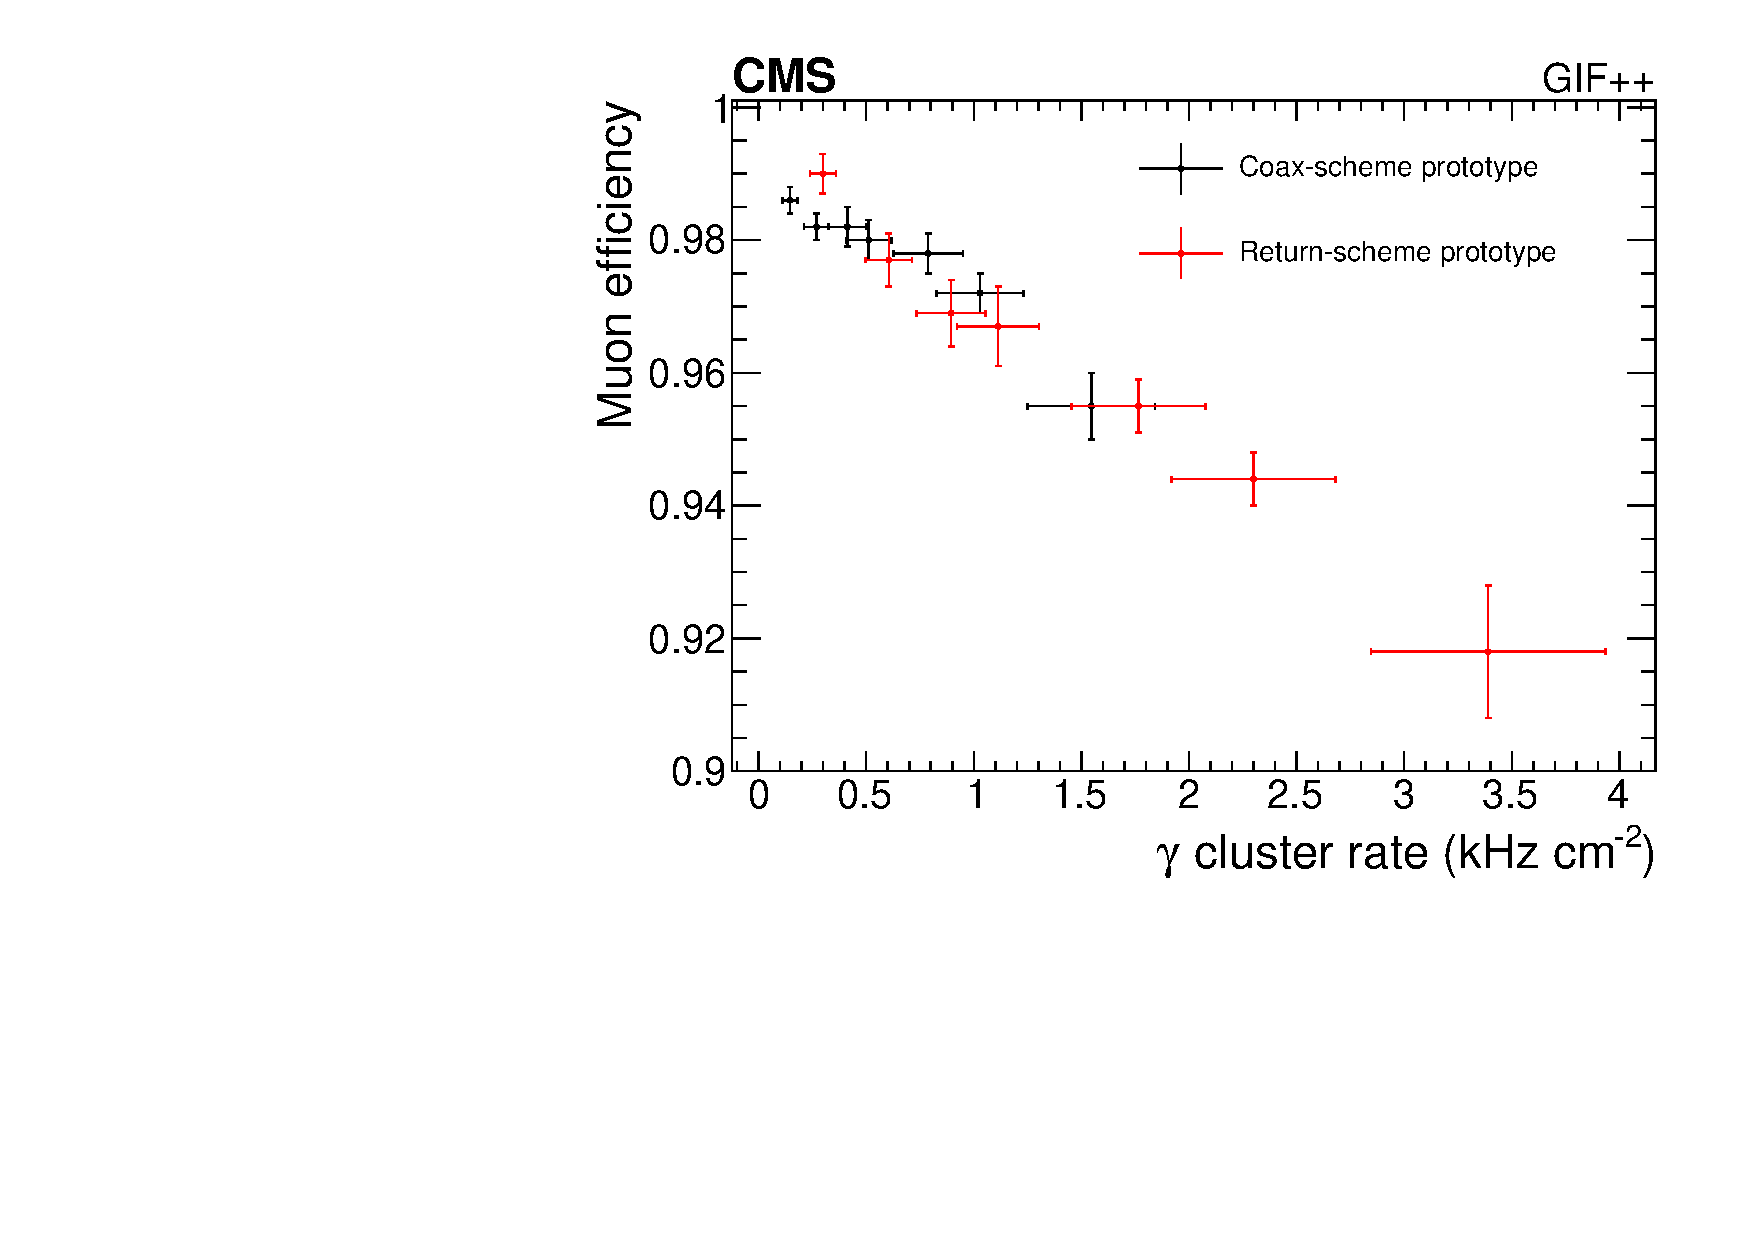
\includegraphics[width=0.40\textwidth]{figs/RETURN_EFFvsRATE.pdf}
    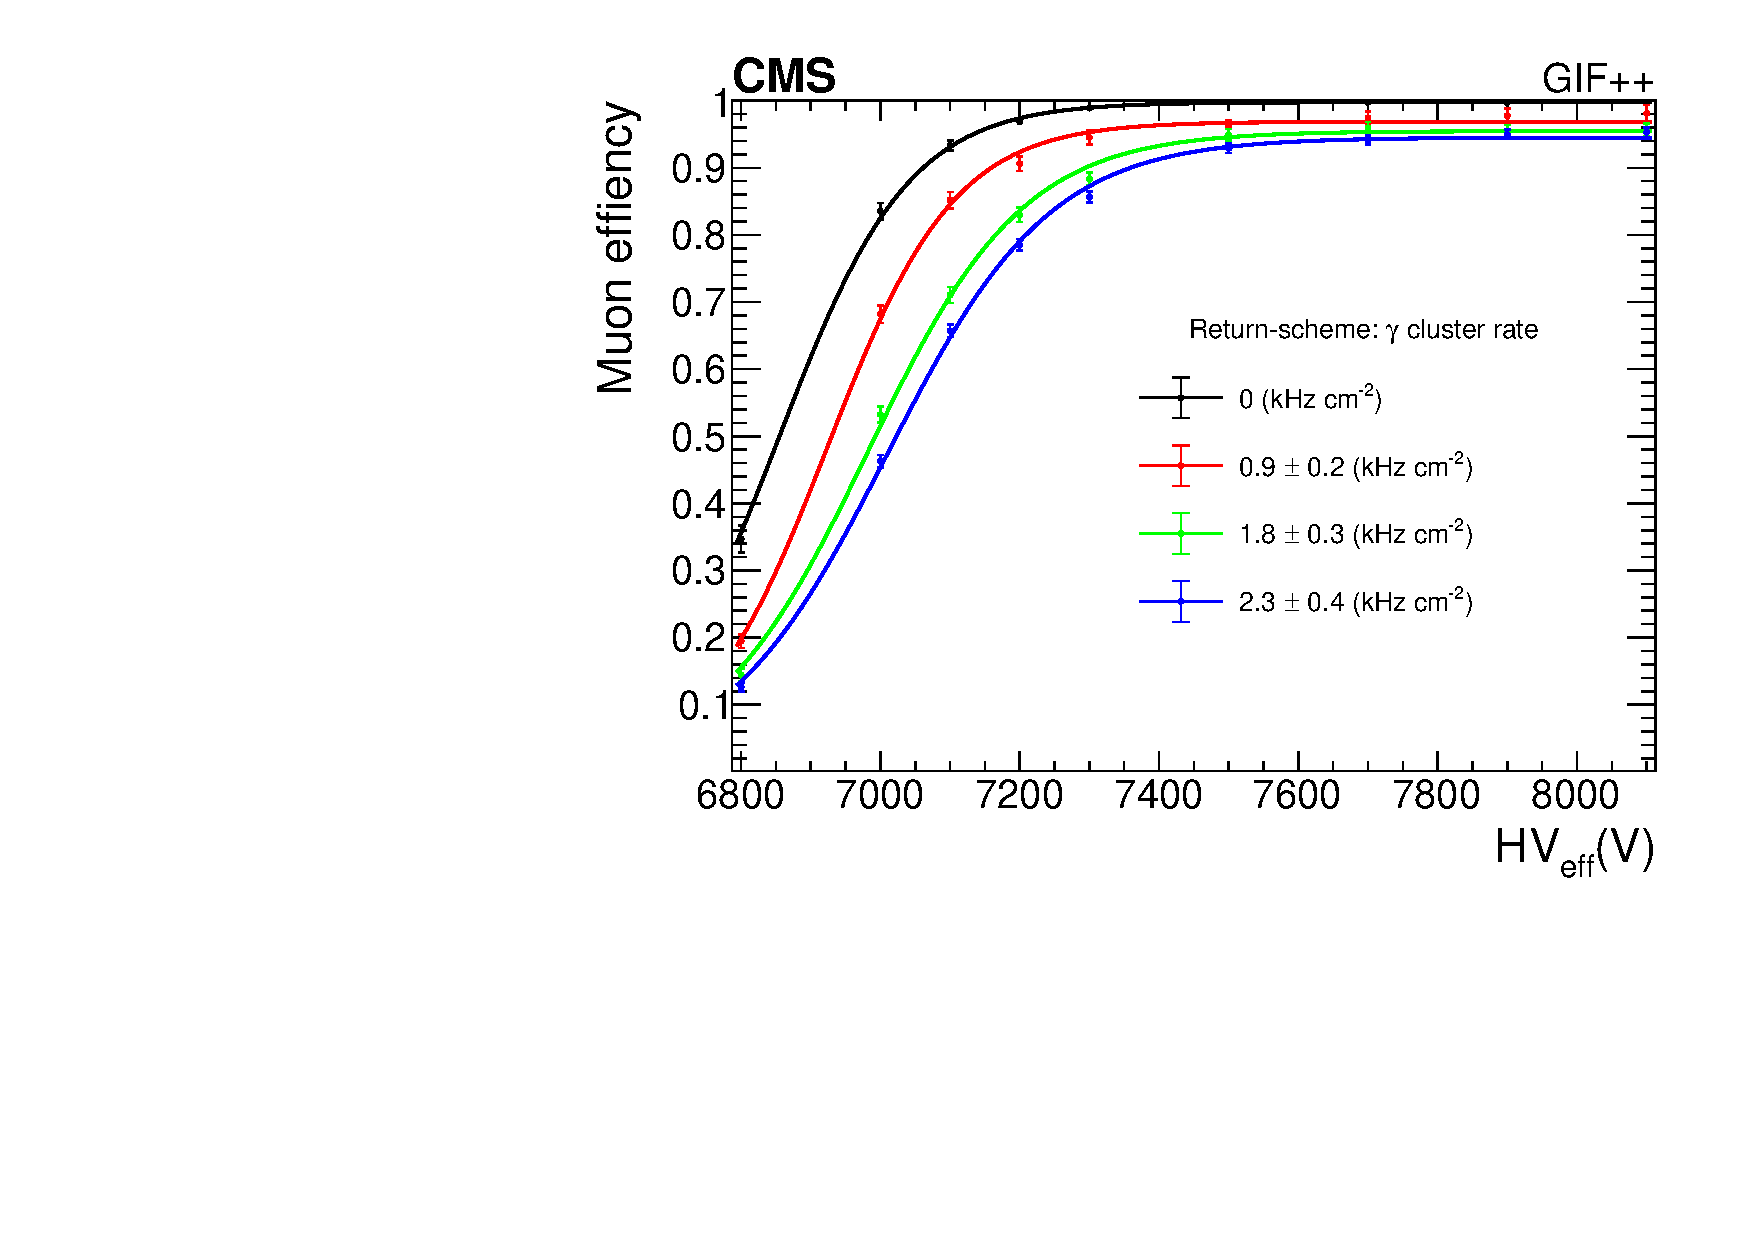
\includegraphics[width=0.40\textwidth]{figs/R_EFFvsHV.pdf}
  \end{center}
 \caption{Efficiency curves as function of the effective high voltage for the Return-scheme prototype shown for different background rates (left). Efficiency at working point for both prototypes at different background rates (right).} \label{fig.eff}
\end{figure}


The space resolution was measured with high precision at the H2 line of the SPS complex with two thin scintillators and a special table (produced by DESY) that allows a horizontal and vertical shift of the chambers with a millimetric precision. We observed in Fig.~\ref{fig.DT} an excellent $\DT$ resolution of the order of $130$\,ns roughly in the center of the chamber ($77$\,cm from high radius) that can be converted into the along-strip space resolution $\Delta y \approx 1.3$\,cm using the formula $\Delta y = v \cdot \Delta {\rm T} / 2$. The speed of the signal propagation $v$ was measured looking at the shift of $\DT$ in ns when the DESY table is moved by $y$\,cm (Fig. \ref{fig.DT}).


\begin{figure}
  \begin{center}
    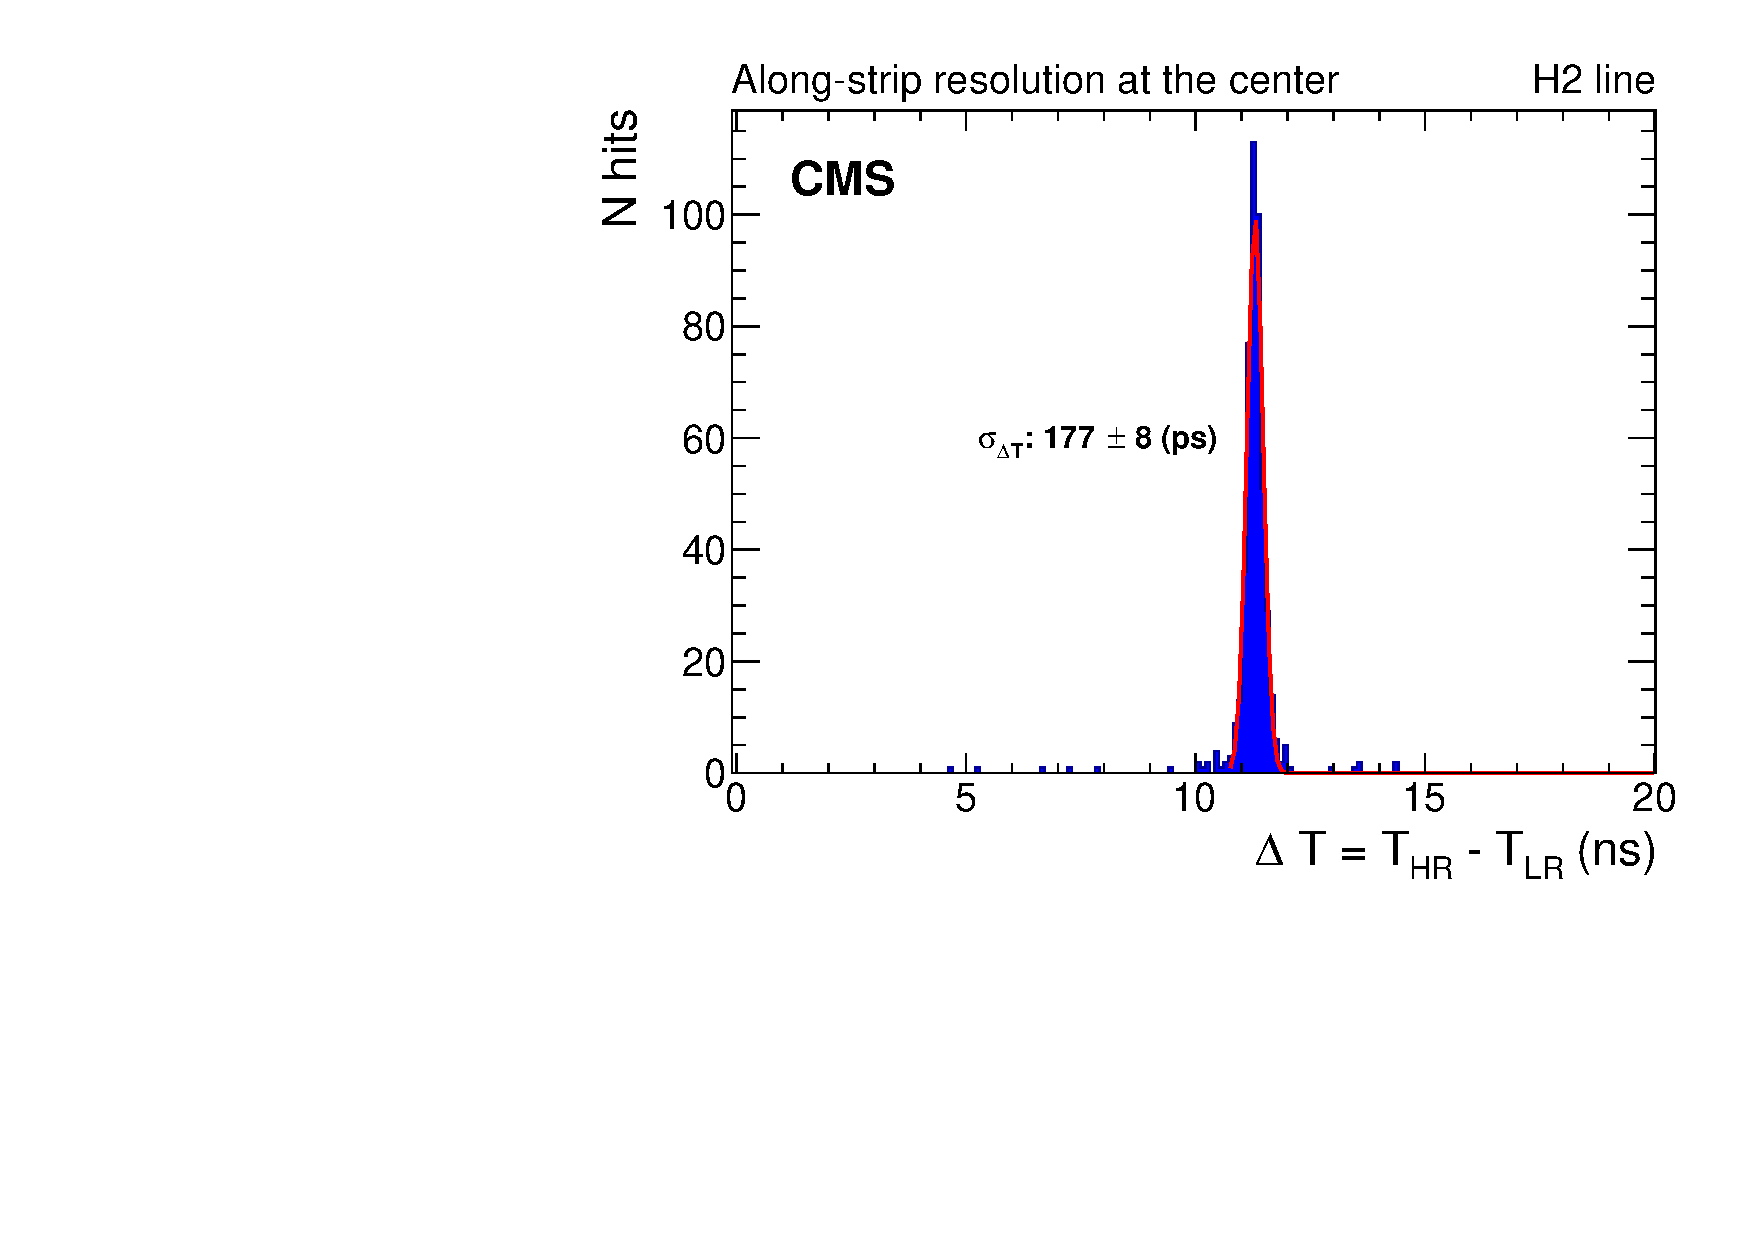
\includegraphics[width=0.40\textwidth]{figs/400.pdf}
    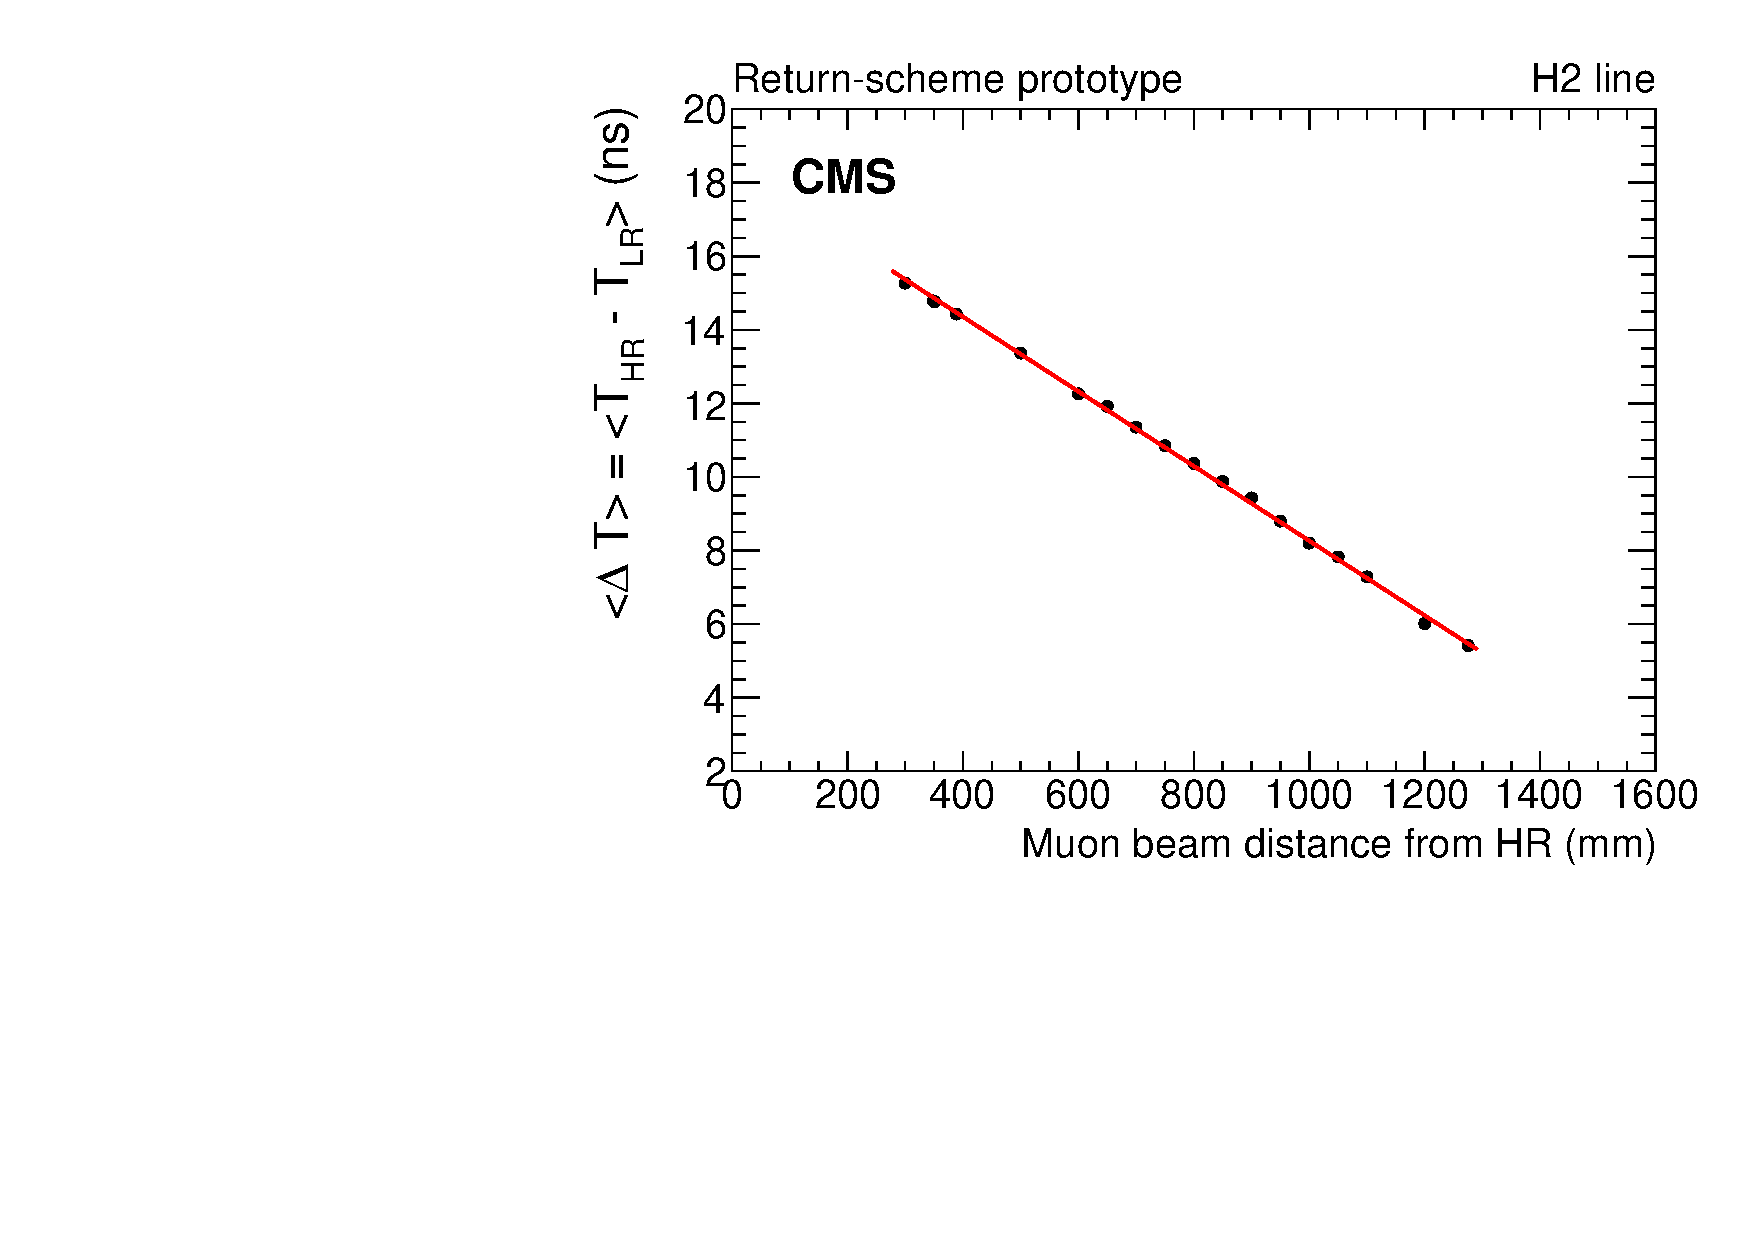
\includegraphics[width=0.40\textwidth]{figs/Position.pdf}
  \end{center}
 \caption{$\DT$ resolution of the Return-scheme prototype at the center of the detector (left). Correlation between the average $\DT$ measurement and the position of the beam with respect to the HR.} \label{fig.DT}
\end{figure}

\section*{Summary}

The iRPC upgrade project was validated in a test beam and fulfills the requirements of operation in the high background rates expected during HL-LHC phase: efficiency above 95\%, space resolution at cm level and absolute time resolution better than $1$\,ns. 

\bibliographystyle{JHEP}
\bibliography{iRPC.bib}

\end{document}
